\section*{\Large{Введение}}
\addcontentsline{toc}{section}{Введение}
При работе с картами на различных устройствах, мы очень редко задумываемся о том, как же, на самом деле,
работает отображение геоданных. Какие технологии используются, чтобы мы смогли увидеть картинку у себя на экране
монитора.

Способ отображения карт можно разбить на 2 больших класса: рендеринг на стороне клиента и рендеринг на стороне
сервера.
В первом случае, в качестве ответа приходят необработанные геоданные и рендеринг осуществляется на машине клиента.
Во втором случае, клиенту уже приходят полностью подготовленные для отображения данных,
которые клиенту следует только отобразить,
никаких математических вычислений ему производить не нужно.

Эти два подхода используются в разных случаях, в зависимости от задач.
При отображении большого объема геоданных следует выбирать подход с рендерингом
на стороне сервера. Это позволит снизить количество данных, передаваемых по сети, снизить нагрузку на
машину клиента, так как не требуется преобразования географических координат в координаты на экране.

Отрендеренные на сервере геоданные называются тайлы. А сам сервер -- тайловым сервером.
Тайлы можно разбить на 2 класса: растровые и векторные. Растровые тайлы используются в качестве
подложки карты(спутниковые снимки и пр.). Их применяют там, где не нужна интерактивность взаимодействия данных
с пользователем. Векторные тайлы -- это подготовленный кусочек геоданных большого объема. Их используют там, где
требуется интерактивность работы с пользователем. Например: пользователь навел на объект мышкой и этот объект подсветился.

\begin{wrapfigure}{r}[0pt]{0.4\textwidth}
    \begin{center}
        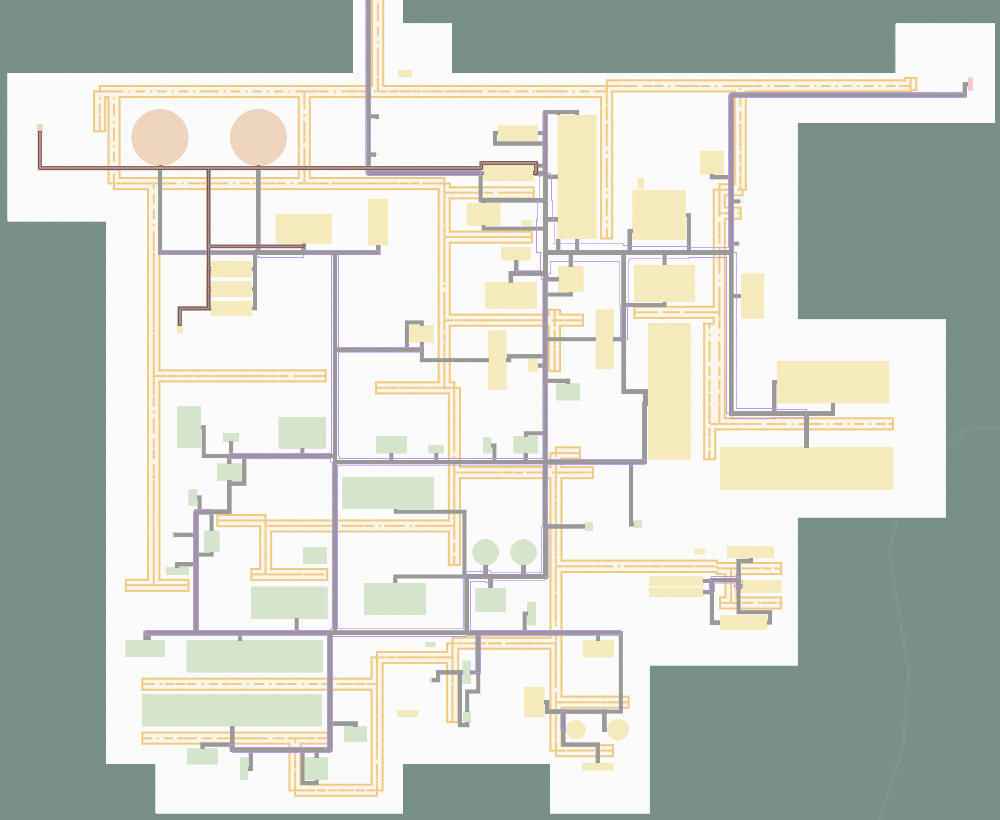
\includegraphics[width=0.8\textwidth]{images/introduction/1}
    \end{center}
    \caption{Пример результата работы}
    \label{pic:problem__site-plan}
\end{wrapfigure}
У нас, как раз, случай, с отображением большого количества геоданных.
Генеральный план площадного объекта содержит большое количество различных зданий, коммуникаций и других объектов
необходимых для функционирования этого площадного объекта(см. рис\ref{pic:problem__site-plan}). И так как мы хотим дать
пользователю взаимодействовать с геоданными, то векторные тайлы позволят решить нам нашу проблему.



